\subsection{Statistics}
\begin{frame}{Statistics}

\begin{figure}[htbp]
	\begin{center}
	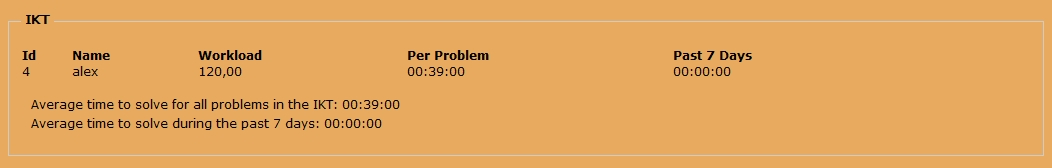
\includegraphics[height=200pt]{input/statistics.jpg}
	%\caption{default}
	%\label{default}
	\end{center}
\end{figure}

\end{frame}

\begin{frame}{Statistics}

\begin{itemize}
\item Current
	\begin{itemize}
	\item Primitive
	\item Based on unsound data
	\end{itemize}
\end{itemize}
\\
\begin{itemize}
\item Potential improvements
	\begin{itemize}
	\item Better data:
		\begin{itemize}
		\item Time solving problems
		\item Type of problem
		\end{itemize}
	\item More factors:
		\begin{itemize}
		\item Time solving problems
		\item ``difficulty'' of the submitter
		\item Working hours of staff
		\end{itemize}
	\end{itemize}
\end{itemize}

\end{frame}